\documentclass[12pt]{report}
\usepackage{caption}
\usepackage{graphicx}
\usepackage{hyperref}
\hypersetup{%
    pdfborder = {0 0 0}
}
\hypersetup{
    colorlinks,
    citecolor=blue,
    filecolor=blue,
    linkcolor=blue,
    urlcolor=blue
}
\renewcommand{\familydefault}{\sfdefault}
\renewcommand{\captionfont}{\small}

\author{Bernd Porr}
\title{Q-learning and deep Q-learning}

\begin{document}

\maketitle

Q-learning ist ein Lernalgorithmus wo ein Agent selbständig
lernt seine Belohnung zu maximieren.

\begin{figure}[!hbt]
\begin{center}
\mbox{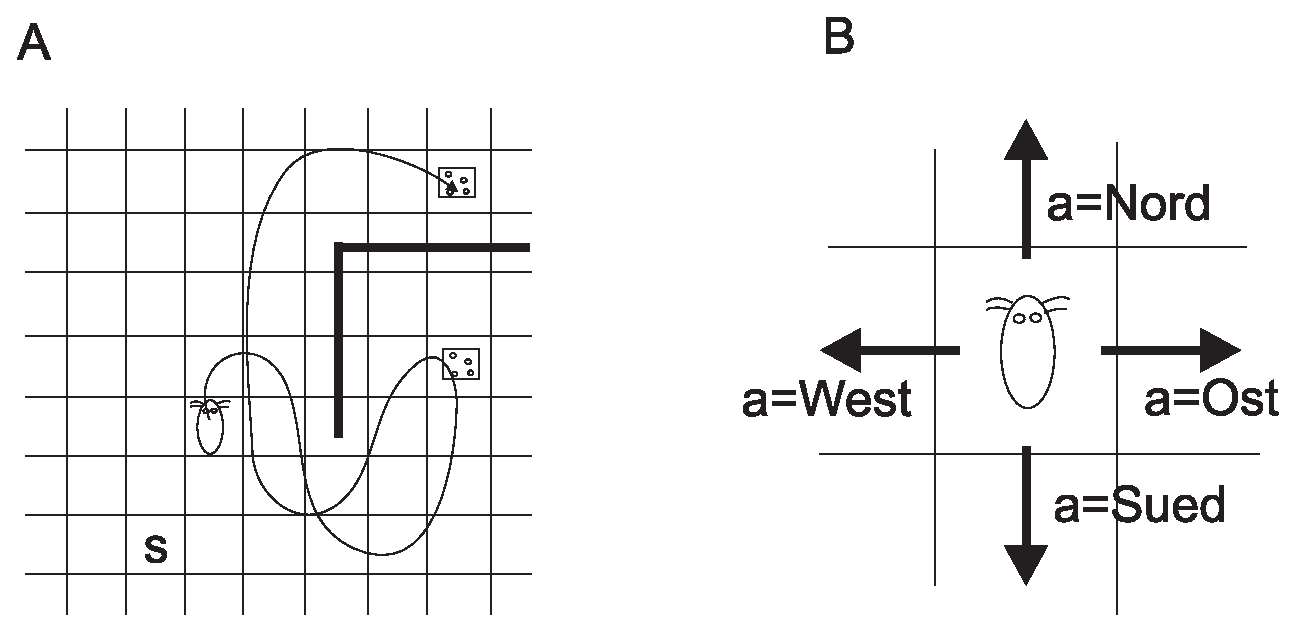
\includegraphics[width=\textwidth]{state_action}}
\end{center}
\caption{Zustandsraum und Aktionen eines autonomen Agenten,
  der Futter sucht.
\label{state_action}}
\end{figure}

Abbildung~\ref{state_action} zeigt eine klassische Welt, in der sich
eine solche Agentin (hier eine Maus) bewegt.  A) zeigt den
Zustandsraum. In diesem Beispiel ist der Zustandsraum 2D, in dem sich
die Agentin bewegen kann. Manche Zustände sind durch Wände verboten und
bei anderen gibt es eine Belohnung (also ``Käse'' gekennzeichnet).
Zustände werden mit $s$ gekennzeichet und wenn sie zum Zeitpunkt
$t$ passieren, dann wird das als $s_t$ gekennzeichet.

B) zeigt die möglichen Aktionen $a$, die die Agentin durchführen kann.
Eine Aktion bewirkt eine Bewegung von einem Zustand $s_t$ zum Zeitpunkt
$t$ zum Zustand $s_{t+1}$. 

\begin{figure}[!hbt]
\begin{center}
\mbox{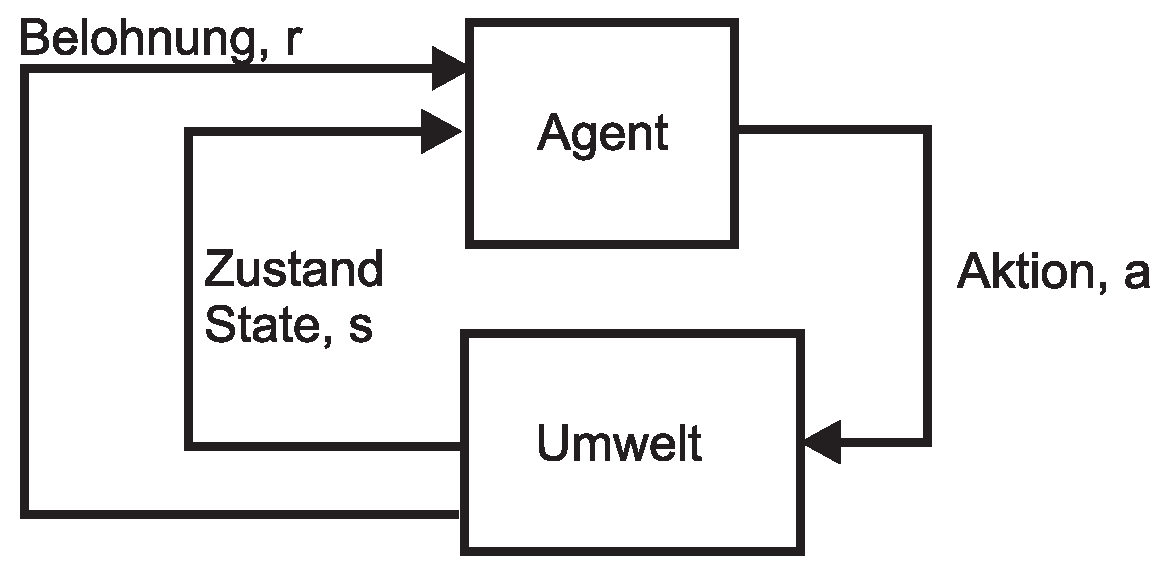
\includegraphics[width=0.75\textwidth]{schleife}}
\end{center}
\caption{Umwelt und Agentin interagieren in einer geschlossenen
  Schleife.
\label{schleife}}
\end{figure}

Abbildung~\ref{schleife} illustriert, wie man die Interaktion
zwischen Agentin und Umwelt als geschlossenes System interpretieren
kann damit die Agentin autonom ist. Jede Aktion $a$ der Agentin
erzeugt einen neuen Zustand $s$ und gegebenenfalls auch eine
Belohnung $r > 0$.

\begin{figure}[!hbt]
\begin{center}
\mbox{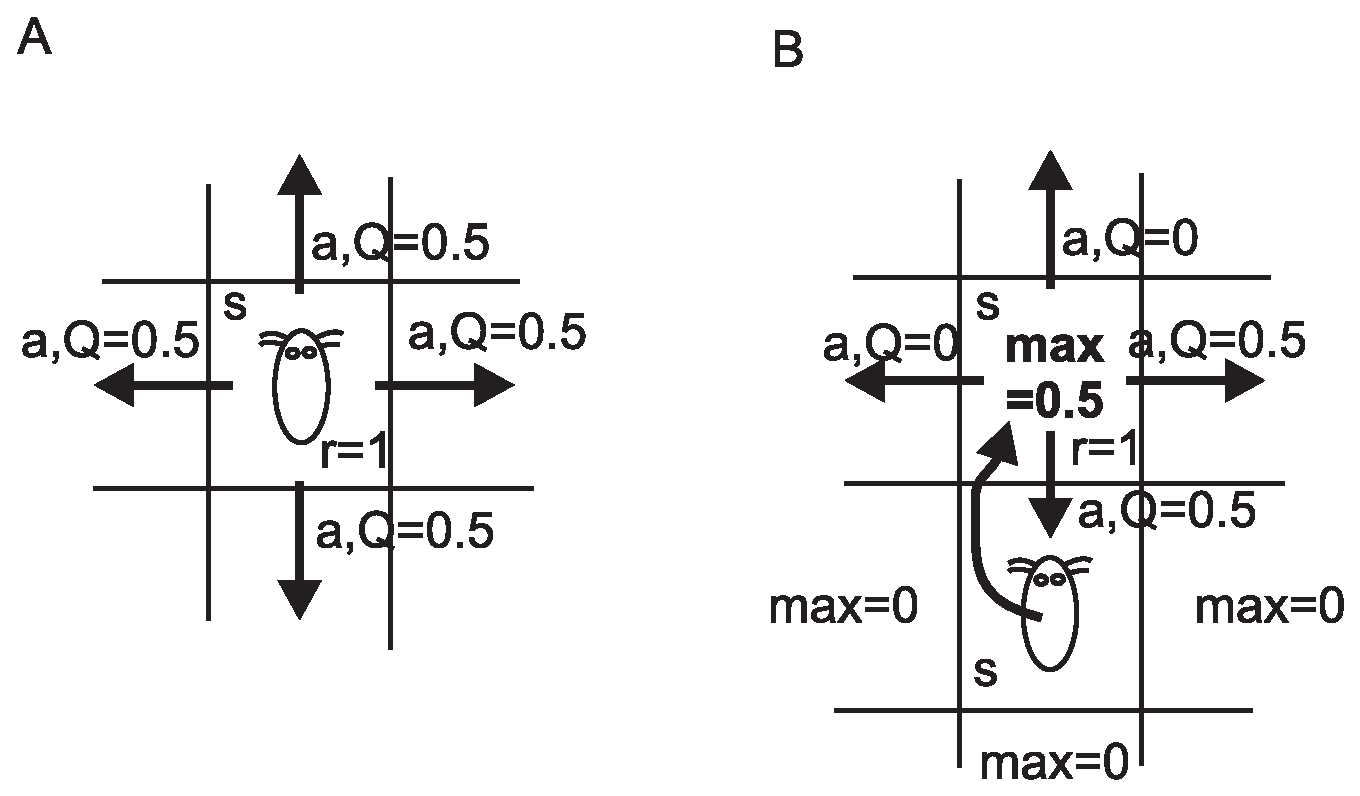
\includegraphics[width=\textwidth]{learning_steps}}
\end{center}
\caption{Lernschritte von Q-learning. A) Die Agentin befindet
  sich direkt auf der Belohnung. Das führt dazu, dass alle
  Q-Werte gleichermassen erhöht werden, z.B. auf $0.5$ mit
  einer Lernrate von $\alpha = 0.5$.
\label{learning_steps}}
\end{figure}

Die Frage stellt sich nun, wie die Agentin von jeder beliebigen Stelle
$s$ die Belohnungen findet. Das wird erreicht, indem jede Aktion $a$
bezueglich eines Zustandes $s$ eine Hilfsvariable erhaelt, die wir
$Q(s,a)$ nennen (siehe Abbildung~\ref{learning_steps}A). In diesem
Beispiel erhaelt jeder Zustand $s$ vier Q-Werte (Nord, West, Ost
und S\"ud). Anfaenglich sind alle Q-Werte null.

Die Q-Werte werden nun mit Hilfe der iterativen Bellman-Formel bestimmt:
\begin{equation}
Q(s,a) \leftarrow Q(s,a) + \alpha \underbrace{\left[ r(s) + \gamma \max_{a^\prime} Q(s^\prime,a^\prime) - Q(s,a) \right]}_{\delta(s,a)} \label{bellit}
\end{equation}
wo $\alpha$ die Lernrate ist und $0 < \gamma < 1$ der ``discount Factor'' der zukünftige Belohnungen abwertet. Hier nehmen
wir einfach an, dass $\alpha = 0.5$ und $\gamma = 1$ ist.

Die Q-Werte werden nun iterativ gelernt, wobei die Agentin Zufallsaktionen $a$ durchführt und dann Q(s,a) aktualisiert wird.
Am Anfang sind all Q-Werte null. Nur die direkte Belohnung kann diesen von Null erhoehen, was in
Abbildung~\ref{learning_steps}A gezeigt wird. Bei einer Lernrate von $\alpha = 0.5$ ergibt das dann fuer alle
Aktionen einen Q-Wert von $0.5$.

Der entscheidende Trick ist aber nun, wenn bei der naechsten Zufallswanderung die simulierte Maus
einen Schritt vor der primaeren Belohnung steht. Nun ist $Q(s,a)$ nicht mehr überall null. Abbildung~\ref{learning_steps}B
zeigt nun die Agentin einen Schritt vor der Belohnung. $Q(s,a)$ ist der Q-Wert \textsl{nach} der Aktion $a$ also einen
Schritt voraus. Das ist alles, was die Agentin ``sehen kann'': einen Schritt voraus und das wird im Sinne von
Q-learning ``Beobachtung'' oder ``Beobachtungshorizont'' genannt. Die Maus schaut also nun in die verschiednen Felder
um sich herum und nimmt den maximalen Q-Wert, vergleicht den mit dem aktuellen Q-Wert und korrigiert dann den aktuellen
Q-Wert anhand der Lernrate. Aus diesem Grunde wird der Term $\delta(s,a)$ auch als Vorhersagefehler identifiziert oder
im Englischen ``Reward Prediction Error'' (RPE).

Das Vorgehen in Abbildung~\ref{learning_steps} wird nun mit der Eq.~\ref{bellit} viele Male wiederholt, bis der
Fehler $\delta$ im Mittel Null ist. Dieser Prozess konvergiert und gibt dann eine Vorhersage der Belohnung
fuer jedes Q in Abhaengigkeit von $s$ und $a$:
\begin{equation}
  Q(s,a) = \sum_{t=0}^T \gamma^t r_t
\end{equation}
wo $T$ die Gesamtzeit ist, die der Agent zur Verfügung gestellt
bekommt, seine Aufgabe zu erledigen.

Wenn $Q(s,a)$ stabil ist, dann kann die Agentin die Belohnung finden, indem sie immer in das Feld springt,
wo die der hoechste Q-Wert ist. Das nennt sich dann eine ``Policy'' oder ``Strategie''. Solch eine Strategie
nennt sich ``gierig'' oder ``greedy'', da sie immer in Richtung der staerksten Belohnung navigiert.

Praktisch gesehen, werden normalwerweise lernen von Q und das Ausfuehren der Strategie gemischt.


\end{document}
